\documentclass{article}
\usepackage[utf8]{inputenc}
\usepackage[margin=1in]{geometry}
\usepackage{amsmath,amsthm,amsfonts,latexsym,amssymb,xcolor}
\usepackage{fancyhdr}
\usepackage{graphicx}
\usepackage{setspace}
\usepackage{hyperref}
\usepackage{tikz}
\usepackage{pgfplots}
\pgfplotsset{compat=1.18}
% Define a custom style for the axes
\pgfplotsset{every axis/.append style={
    axis lines=middle, % No grid or box surrounding axes
    ticks=none, % Hide tick marks and labels
}}
\usepackage{imakeidx}
\makeindex
\usepackage[skip=\medskipamount]{parskip}
\pagestyle{fancy}
\setlength{\headheight}{25pt}
\setlength{\parindent}{0pt}

\newcommand{\interior}{\text{int}}
\newcommand{\cl}{\text{cl}}
\newcommand{\bd}{\text{bd}}
\newcommand{\R}{\mathbb{R}}
\newcommand{\N}{\mathbb{N}}
\newcommand{\Q}{\mathbb{Q}}
\newcommand{\Z}{\mathbb{Z}}
\newcommand{\norm}[1]{\lVert #1 \rVert}
\newcommand{\sol}{\bigskip \bigskip \emph{Solution.} \bigskip}
\newcommand{\pf}{\bigskip \bigskip \emph{Proof.} \bigskip}
\newcommand{\keyword}[1]{\textit{\textbf{#1}}\index{#1}}

% Using amsthm package
\newtheorem{theorem}{Theorem}
\newtheorem{lemma}{Lemma}
\newtheorem{claim}{Claim}


\newtheorem{assumption}{Assumption}

\theoremstyle{definition}
\newtheorem{definition}{Definition}
\newtheorem{remark}{Remark}
\newtheorem{ex}{Example}

\title{Lecture 1: Proofs, Metric Spaces, Topology}
\author{Originally written by Mauricio Caceres Bravo\\Revised by Cole Davis\\Webpage: \href{https://cj-davis99.github.io/math-camp.html}{cj-davis99.github.io}}
\date{August 13, 2024}

\linespread{1.25}

\begin{document}
\lhead{Math Camp \\ August 13, 2024} 
\rhead{Lecture 1 \\ \leftmark}
\maketitle
\tableofcontents
\newpage
\section*{Notation}
\begin{itemize}
    \item $\wedge$ is a logical ``and''
    \item $\mid$ is a logical ``or''
    \item $\neg$ is a logical negation
    \item $\forall$ translates to ``for all''
    \item $\exists$ translates to ``there exists''
    \item $\N = \{1,2, \hdots\}$ is the set of natural numbers
    \item $\Z = \{\hdots, -1, 0, 1, \hdots \}$ is the set of integers
    \item $\Q = \left\{ p/q : p \in \Z \text{ and } q \in \Z\backslash\{0\} \right\}$ is the set of rational numbers
    \item $\R$ is the set of real numbers
    \item If $S$ is a set and $n\in \N$, then $S^n$ is the $n^{\text{th}}$ order Cartesian product of $S$. E.g., $S^2 = S \times S$ 
\end{itemize}
\newpage
\section{Proofs and Logic}
Math is a language: It should be possible to express anything you want in math, as you would in English or any other language. However, there are many things that are easier to express in math (just like many things are easier to express in English). One thing that is easier to do in math are proofs.

\subsection{If $P$ then $Q$}
Suppose $P$ and $Q$ are two \keyword{logical statements}; that is, suppose we can objectively claim that $P$ is true or false (but not both) and we can do the same for $Q$. 
\begin{itemize}
    \item Logically, we say that $P \implies Q$, that is, ``$P$ implies $Q$''. It's also common for people to say ``$P$ is a sufficient condition for $Q$'' and ``$Q$ is a necessary condition of $P$''.
    \begin{figure}[h]
      \centering
      \begin{tikzpicture}[scale=1]
        \draw [->, >=latex]
          (-2, 0.75) to[bend right=15] (-0.75, 0.25)
          node[above] at (-2, 0.75) {$P$ is sufficient for $Q$};
        \draw [->, >=latex]
          (2, -0.75) to[bend right=15] (0.75, 0.25)
          node[below] at (2, -0.75) {$Q$ is necessary for $P$};
        \node[above] at (0, 0) {$P \implies Q$};
      \end{tikzpicture}
    \end{figure}
    
    \item Graphically, we say that $P\subseteq Q$
    \begin{figure}[h]
      \centering
      \begin{tikzpicture}[scale=1]
        \draw (0, 0) circle [radius=1.5];
        \draw (-0.5, -0.5) circle [radius=0.5];
        \node[above] at (-0.5, -0.5) {$P$};
        \node[above] at (0.5, 0.5) {$Q$};
      \end{tikzpicture}
    \end{figure}
    
    \item Logical conditions can also be defined using a \keyword{truth table}. In a truth table, we list out all the possible combinations of logical values that $P$ and $Q$ could take, and then we can assert when the logical operation enacted on the statements holds. For example, we can use a truth table to figure out when $P \implies Q$ is a logically valid statement. If T means true and F means false, then Table~\ref{tab:P_Q_logic} displays all the possible logical combinations the statements $P$ and $Q$ can take. 
    \begin{table}[ht]
        \centering
        \begin{tabular}{c c c}
             $P$ & $\implies$ & $Q$\\\hline
             T & & T \\
             T & & F \\
             F & & T \\
             F & & F \\
        \end{tabular}
        \caption{All logical combinations of $P$ and $Q$}
        \label{tab:P_Q_logic}
    \end{table}
    Intuitively, $P \implies Q$ should mean that whenever $P$ is true, $Q$ is also true. We illustrate this in Table~\ref{tab:P_imp_Q}.
    \begin{table}[ht]
        \centering
        \begin{tabular}{c c c}
             $P$ & \color{blue}$\implies$ & $Q$\\\hline
             T & \color{blue}T & T \\
             T & \color{blue}F & F \\
             F & \color{blue}T & T \\
             F & \color{blue}T & F \\
        \end{tabular}
        \caption{$P\implies Q$}
        \label{tab:P_imp_Q}
    \end{table}
    Note that whenever $P$ is false, the statement $P\implies Q$ trivially holds true. 
    \begin{ex}\label{ex:P_imp_Q}
        Define $P$ and $Q$ as the following statements:
        \begin{center}
            $P$: I get A's in all of the first-year courses.\\
            $Q$: Kareen Rozen buys me a car. 
        \end{center}
        If the statement $P\implies Q$ is true, then there are 3 possible states of the world:
        \begin{enumerate}
            \item I get all A's in the first-year courses and Kareen buys me a car
            \item I do not get all A's in the first-year courses and Kareen does not buy me a car
            \item I do not get all A's in the first-year courses and Kareen buys me a car
        \end{enumerate}
        If the statement $P\implies Q$ is false (which is the unfortunate reality you should expect), then even if I get all A's in the first-year courses, Kareen does not buy me a car. 
    \end{ex}
    \begin{remark}
        The $P$ statement in Example~\ref{ex:P_imp_Q} is actually a collection of logical statements strung together with the logical ``and'' operation. That is, we can equivalently write $P$ as follows
        \begin{center}
            P: I get an A in micro 1 and I get an A in macro 1 and...
        \end{center}
        There are 3 primitive (i.e., base level) logical operations: ``and'', ``or'', and ``not''. We will write these primitive logical operations (respectively) as $P \wedge Q$, $P \mid Q$, and $\neg P$. Tables~\ref{tab:P_and_Q}, \ref{tab:P_or_Q}, and \ref{tab:not_P} are the relevant truth tables for the respective primitive logical operations. 
        \begin{table}[ht]
        \centering
        \begin{tabular}{c c c}
             $P$ & \color{blue}$\wedge$ & $Q$\\\hline
             T & \color{blue}T & T \\
             T & \color{blue}F & F \\
             F & \color{blue}F & T \\
             F & \color{blue}F & F \\
        \end{tabular}
        \caption{$P\wedge Q$}
        \label{tab:P_and_Q}
    \end{table}
    \begin{table}[ht]
        \centering
        \begin{tabular}{c c c}
             $P$ & \color{blue}$\mid$\color{black} & $Q$\\\hline
             T & \color{blue}T & T \\
             T & \color{blue}T & F \\
             F & \color{blue}T & T \\
             F & \color{blue}F & F \\
        \end{tabular}
        \caption{$P\mid Q$}
        \label{tab:P_or_Q}
    \end{table}
    \begin{table}[ht]
        \centering
        \begin{tabular}{c c}
             \color{blue}$\neg$ & $P$ \\\hline
             \color{blue}F & T  \\
             \color{blue}T & F  \\
        \end{tabular}
        \caption{$\neg P$}
        \label{tab:not_P}
    \end{table}
    \end{remark}
\end{itemize}

Note that $P \implies Q$ does not (generally) mean $Q \implies P$. This can be seen via a truth table, but can also be illustrated using the setup of Example~\ref{ex:P_imp_Q}: suppose $P\implies Q$ is a true statement, I don't get straight A's in the first-year courses, and Kareen buys me a car. This is a logically consistent state of the world given that $P\implies Q$ is a true statement; however, it would not be a logically consistent state of the world if instead $Q\implies P$ because $Q$ would be true, but $P$ would be false. Thus, $P\implies Q$ need not mean that $Q \implies P$. 

Although $P\implies Q$ is not logically equivalent to $Q \implies P$, the statement $\neg Q \implies \neg P$ is logically equivalent to $P \implies Q$ and is called the contrapositive of the statement $P\implies Q$. To see that they are equivalent statements, consider the truth table illustrated in Table~\ref{tab:contrapositive} (compared with Table~\ref{tab:P_imp_Q}).
\begin{table}[ht]
        \centering
        \begin{tabular}{c c c}
             $\neg P$ & \color{blue}$\Longleftarrow$\color{black} & $\neg Q$\\\hline
             F & \color{blue}T & F \\
             F & \color{blue}F & T \\
             T & \color{blue}T & F \\
             T & \color{blue}T & T \\
        \end{tabular}
        \caption{$\neg Q \implies \neg P$}
        \label{tab:contrapositive}
    \end{table}

\subsection{Proof Strategies}
\begin{enumerate}
    \item \keyword{Direct proof}: Show $P\implies Q$; that is, find some path of logical statements that leads from $P$ to $Q$. To illustrate a direct proof, we need the following definitions:
    \begin{definition}\label{def:parity}
        We say that an integer $n$ is \keyword{even} if there exists a $k\in \Z$ such that $n = 2k$. Similarly, we say that an integer $m$ is \keyword{odd} if there exists an $j\in \Z$ such that $m = 2j + 1$. 
    \end{definition}
    Consider the claim below:
    \begin{claim}
        If $n\in Z$ is even, then $p\cdot n$ is even for any $p\in \Z$. 
    \end{claim}
    \begin{proof}
        Suppose $n\in\Z$ is even. By Definition~\ref{def:parity}, we know that there exists a $k\in \Z$ such that $n = 2k$. Then we can write
        \begin{equation*}
            p n = p (2n) = 2 (pn)
        \end{equation*}
        We know that $pn \equiv q \in \Z$. Thus, 
        \begin{equation*}
            pn = 2q
        \end{equation*}
        Therefore, $pn$ is even by Defintion~\ref{def:parity}.  
    \end{proof}
    \item \keyword{Contrapositive}: Show $\neg Q \implies \neg P$. This is very similar to a direct proof, but often it is useful to rephrase what we want to show in its contrapositive form. Further, texts will, at times, proceed by contrapositive without making explicit mention that is what they are doing. We illustrate a contrapositive proof technique by proving the following claim:
    \begin{claim}\label{claim:sqrt2_irrational_lem}
        Suppose $p\in \Z$. If $p^2$ is even, then $p$ is even.
    \end{claim}
    \begin{proof}
        Suppose $p\in Z$. Note that every integer is either even or odd (this can be proven). Thus, the negation of the statement:
        \begin{center}
            $P(p)$: $p$ is even 
        \end{center}
        is
        \begin{center}
            $\neg P(p)$: $p$ is odd
        \end{center}
        
        Suppose $p$ is odd. Then there exists a $k\in \Z$ such that 
        \begin{equation*}
            p = 2k+1
        \end{equation*}
        Squaring both sides of the equation above yields
        \begin{align*}
            p^2 &= (2k+1)^2 \\
            &= 4k^2 + 4k + 1 \\
            &= 2(2k^2 + 2k) + 1
        \end{align*}
        Let $\ell = 2k^2 + 2k$. We know that $\ell\in\Z$. Therefore, 
        \begin{equation*}
            p^2 = 2\ell + 1
        \end{equation*}
        so $p^2$ is odd by Definition~\ref{def:parity}. 
    \end{proof}

    \item \keyword{Contradiction}: A contradiction proof can be used to prove more than just conditional statements (i.e., if $P$ then $Q$). The basic structure of a contradiction proof is to assume that the statement you wish to be true is actually false, and then derive a logical contradiction (i.e., reach a conclusion that you know to be incorrect). We illustrate a contradiction proof via a famous example:
    \begin{claim}\label{claim:sqrt2_irrational}
        $\sqrt{2}$ is irrational
    \end{claim}
    Before we move forward with the proof, we first note that an irrational number is any number that is not in $\Q$; that is, $x$ is irrational if for any $p\in \Z$ and $q\in \Z \backslash \{0\}$, 
    \begin{equation*}
        x \neq \frac{p}{q}
    \end{equation*}
    \begin{definition}\label{def:co-prime}
        Suppose $p,q\in \Z$. We say that $p,q$ are \keyword{co-prime} if their only mutual positive integer divisor is 1.  
    \end{definition}
    We are ready now to prove Claim~\ref{claim:sqrt2_irrational}:
    \begin{proof}[Proof for Claim~\ref{claim:sqrt2_irrational}]
        For the sake of contradiction, suppose that $\sqrt{2}\in \Q$. Then there exists 2 co-prime integers $p,q$ (with $q\neq 0$)\footnote{Let $\sqrt{2} = \widetilde{p} / \widetilde{q}$ for any $\widetilde{p}, \widetilde{q}\in \Z$ (with $\widetilde{q}\neq 0$) and let $m$ be the product of all their co-factors; $p \equiv \widetilde{p} / m, q \equiv \widetilde{q} / m$ gives $\sqrt{2} = p / q$ with $p, q$ co-prime.} such that 
        \begin{equation*}
            \sqrt{2} = \frac{p}{q}
        \end{equation*}
        Squaring both sides of the equation above gives us
        \begin{equation*}
            2 = \frac{p^2}{q^2}
        \end{equation*}
        (we know that $\frac{p^2}{q^2} \geq 0$, so we need not consider the possibility that $\frac{p^2}{q^2} = -2$). Simple arithmetic yields
        \begin{equation}\label{eq:sqrt(2)_irrational_eq}
            2q^2 = p^2
        \end{equation}
        Thus, $p^2$ is even. By Claim~\ref{claim:sqrt2_irrational_lem}, it must be that $p$ is even; that is, there exists a $k\in\Z$ such that 
        \begin{equation*}
            p = 2k
        \end{equation*}
        Plugging this into \eqref{eq:sqrt(2)_irrational_eq} gives us 
        \begin{equation*}
            2q^2 = 4k^2 \Rightarrow q^2 = 2k^2
        \end{equation*}
        Thus, $q^2$ is even which implies that $q$ is even by Claim~\ref{claim:sqrt2_irrational_lem}. But then $p$ and $q$ are both divisible by 2, contradicting $p$ and $q$ being co-prime. 
    \end{proof}

    \item \keyword{Induction}: We want to say something about statements that can be indexed by the natural numbers. Using induction we do that in two steps:
    \begin{enumerate}
      \item[a)] Prove the \keyword{base step}, $P(1)$, is true.

      \item[b)] Prove the \keyword{inductive step}, $P(k) \implies P(k + 1)$, is true (i.e. assume $P(k)$ is true and show $P(k + 1)$).
  \end{enumerate}
  We illustrate this proof technique by proving the following claim:
  \begin{claim}
      The sum of the first $k$ positive odd numbers is odd; that is, 
      \begin{equation*}
          \sum_{i=1}^k (2i - 1) = k^2
      \end{equation*}
  \end{claim}
  \begin{proof}
      For the base step, we can see $1 = 1^2$. For the inductive step, assume $P(k)$ is true and show $P(k + 1)$:
          \begin{equation*}
              \sum^{k + 1}_{i = 1} (2i - 1)
            =
            \sum^{k}_{i = 1} (2i - 1)
            +
            2(k + 1) - 1
            \stackrel{!}{=}
            k^2
            +
            2k
            +
            1
            =
            (k +  1)^2
          \end{equation*}
          where $\stackrel{!}{=}$ is true by the inductive step assumption (i.e., $P(k)$ true means $\sum^{k}_{i = 1} (2i - 1) = k^2$).
  \end{proof}
  \begin{remark}
      The base step need not be the $k=1$ case in general (e.g., \href{https://en.wikipedia.org/wiki/Mathematical_induction#Base_case_other_than_0_or_1}{visit this link}); however, it is required that there is a definitive starting point, so the base step can be performed. Induction proofs also require a natural iteration of possible scenarios, so the inductive step can be performed. By the end of this set of lecture notes, we can be more mathematically explicit about what type of problems can be proven using induction. 
  \end{remark}
\end{enumerate}

\section{Functions}
We will not delve into set theory. Intuitively, we can think of a set as a collection of (unique) elements, and we can think of functions as rules that associate every element in one set with an element in another set.\footnote{Formally, we can define a function $f$ from $X$ to $Y$ as a binary relation s.t. $f \subseteq (X \times Y)$ and for each element $x \in X$ there is one (and only one) element $y \in Y$ s.t. $(x, y) \in f$ (though for each element in $y$ there may be some $z \ne x$ s.t. $(z, y) \in f$). Chapter 1 of Ok has a rigorous treatment of functions following an introduction to set theory.}
\begin{definition}\label{def:function}
     We say $f$ is a \keyword{function} with \keyword{domain} $X$ mapping to a \keyword{co-domain} $Y$ if for every element $x\in X$ there exists a $y\in Y$ such that $f(x) = y$. We write $f:X\to Y$, and for any $S\subseteq X$
    \begin{equation*}
        f(S) = \left\{ y \in Y : \exists x\in X ~~\text{s.t.}~~ f(x) = y \right\}
    \end{equation*}
    is the \keyword{image} of $S$ under $f$. The image of the domain, $f(X)$, is called the \keyword{range}. 
\end{definition}
\begin{definition}
    If $f:X\to Y$, then for any $S\subseteq Y$ the \keyword{pre-image} (or \keyword{inverse image}) of $S$ is 
    \begin{equation*}
        f^{-1}(S) = \left\{
      x \in X: \exists y \in Y ~~\text{s.t.}~~ f(x) = y
    \right\}
    \end{equation*}
\end{definition}
\begin{remark}
  The inverse image is distinct from the concept of an inverse function. A function is invertible if $\exists g:Y\to X$ s.t. $f(x) = y \iff g(y) = x$; this is also denoted $g = f^{-1}$ because the image of the inverse is the inverse image. However, functions need not be invertible, while the inverse image is always defined.
\end{remark}

In general it need not be the case that $f(X) = Y$, since some points of $Y$ might not be mapped into. Further, a single point in $Y$ might be the mapping of several points in $X$. We have some special interest in functions for which that is not the case.
\begin{definition}\label{def:injective}
  A function $f: X \to Y$ is \keyword{injective} (or one-to-one) if $f(x) = f(y) \implies x = y$.
\end{definition}

\begin{definition}\label{def:surjective}
  $f$ is \keyword{surjective} (or onto) if $f(X) = Y$.
\end{definition}

\begin{definition}\label{def:bijective}
  $f$ is \keyword{bijective} or a bijection if it is injective and surjective.
\end{definition}

We can mathematically express Definitions~\ref{def:function}, \ref{def:injective}, \ref{def:surjective}, and \ref{def:bijective} (respectively) as
\begin{itemize}
    \item We say $f$ is a function (or is \keyword{well-defined}) if for any $x,x'\in X$, $x = x' \implies f(x) = f(x')$

    \item We say $f$ is an injection if for any $x,x'\in X$, $f(x) = f(x') \implies x = x'$

    \item We say $f$ is a surjection if for any $y \in Y$, there exists an $x \in X$ such that $f(x) = y$
    \item We say $f$ is a bijection if for any $y\in Y$, there exists a unique $x \in X$ such that $f(x) = y$
\end{itemize}
It is expected that first-year graduate students have internalized\footnote{When I say \textit{internalize} a concept, I don't mean memorize; rather, I am saying that you should develop a fundamental understanding of the concept.} the subtlety of these different statements. 

\section{Countability}
\begin{definition}[countability]\label{def:lecture1_countable}
  A set $X$ is \keyword{countably infinite} or \keyword{countable} if $\exists$ a bijection from $X$ to the natural numbers $\N$.
\end{definition}
We make a distinction between finite and countable (note finite sets are not countable by the above definitions; however, it is common to not be very strict in distinguishing between finite and countable sets). Some examples of countably infinite sets:
\begin{enumerate}
  \item $\mathbb{N}$ is countable since a bijection from $\mathbb{N} \to \mathbb{N}$ is given by the identity $f(x) = x$.

  \item $\mathbb{Z}$ is countable. This is slightly more complicated but we can enumerate all the integers:
    \[
      \left\{0, 1, -1, 2, -2, \ldots\right\}
    \]

    This is the enumeration given by the bijection $f:\Z \to \N$ defined via the following mapping: 
    \begin{equation*}
        f(z) = \begin{cases}
            2z & z > 0 \\
            2|z| + 1 & z \leq 0
        \end{cases}
    \end{equation*}
\end{enumerate}

Is $\Q$ countable? Is $\R$? The answers are yes and no, respectively, but the arguments are more nuanced.

\begin{claim}\label{claim:Q_countable}
  $\Q$ is countable.
\end{claim}
Before we walk through the argument for Claim~\ref{claim:Q_countable}, we first prove the following lemma:
\begin{lemma}\label{lem:injection_countable}
    Let $X$ be a set. If the cardinality of $X$ is not finite and there exists an injection $f:X \to \N$, then $X$ is countable. 
\end{lemma}
\begin{proof}
    Suppose $f(X) \subseteq \N$, $f$ is injective, and the cardinality of $X$ (i.e., the number of elements in $X$) is not finite. We can enumerate the range of $f$ as follows:
    \begin{equation*}
        f(X) = \left\{ n_1, n_2, n_3, \hdots \right\}
    \end{equation*}
    Since $f$ is injective, for any $n_i \in f(X)$, there exists a unique $x_{n_i} \in X$ such that $f(x_{n_i}) = n_i$. Define $g:X\to \N$ via the following mapping:
    \begin{equation*}
        g(x_{n_i}) = i
    \end{equation*}
    and note that $g$ is a bijection. Therefore, $X$ is countable. 
\end{proof}

An immediate corollary of Lemma~\ref{lem:injection_countable} is that if $X$ is countable and $S \subseteq X$, then $S$ is countable (or finite), as the bijection defined over $X$ would still be an injection when restricted to $S$. Now to show $\Q$ is countable, consider $g(p, q) = p / q$ defined over the set $\Z \times (\Z \setminus \{0\})$. We can see $\Q = g(\Z \times (\Z \setminus \{0\}))$, and $g^{-1}(\Q) \subseteq \Z \times \Z$. If we can show $\Z \times \Z$ is countable, it should follow $\Q$ is countable.

\begin{proof}[Proof for Claim~\ref{claim:Q_countable}]
    Take any sets $P, Q$ countable; we can enumerate their elements as
  \begin{equation*}
    P = \left\{ p_1, p_2, \ldots \right\}
    \quad
    \text{and}
    \quad
    Q = \left\{ q_1, q_2, \ldots \right\}
  \end{equation*}

  and we can enumerate their Cartesian product as
  \begin{equation*}
      \begin{matrix}
      Q \times P & p_1 & p_2 & p_3    & p_4    & \ldots \\
      q_1        & 1   & 3   & 6      & 10     &        \\
      q_2        & 2   & 5   & 9      &        &        \\
      q_3        & 4   & 8   & \ddots &        &        \\
      q_4        & 7   &     &        & \ddots &        \\
      \vdots
    \end{matrix}
  \end{equation*}
  meaning $P \times Q$ is countable. The bijection that corresponds to that table is
  \begin{align*}
    f(p_i, q_j) = \dfrac{(i + j - 1)(i + j)}{2} - (i - 1)
  \end{align*}
\end{proof}

\begin{claim}
    $\R$ is not countable. 
\end{claim}
\begin{proof}
    We proceed by contradiction. Suppose $\R$ is countable, so we can enumerate its elements as $\R = \{r_1, r_2, \ldots\}$. The decimal representation of each element in $\R$ is then
  \begin{align*}
    r_1 & = N_1.x_{11}x_{12}x_{13}\ldots \\
    r_2 & = N_2.x_{21}x_{22}x_{23}\ldots \\
    r_3 & = N_3.x_{31}x_{32}x_{33}\ldots \\
    \vdots
  \end{align*}

  where $N_i \in \Z$ and $x_{ij} \in \{0, \ldots, 9\}$. Take $y = N.y_1y_2y_3\ldots$ s.t. $y_i \neq x_{ii}$ and $y$ doesn't have an alternative representation (so $y$ doesn't end in all $0$s or all $9$s; but we can do this, since for any $x_{ii}$ we have $7$ numbers to choose from other than $0, 9$, or $x_{ii}$). $y \in \R$ but $y \neq r_j$ for any $j$, contradiction. (Georg Cantor, the mathematician who originally proved this result, actually did this proof for just the real interval $[0, 1]$; can you see why that's sufficient?)
\end{proof}

Why doesn't this proof work for $\Q$?\footnote{If we try to use that same proof to show $\Q$ is not countable there is actually no guarantee that the number $y$ we construct will be an element of $\Q$. We have already established there are numbers that are not in $\Q$, whereas $\R$ is actually defined to be complete (this is a formal term, but intuitively it means that $\R$ has \textit{all} the numbers).}

\begin{remark}
  The finite Cartesian product of countable sets is countable, which we can show by induction. We walk through a simpler claim: if $P$ is countable, then $P^N$ is also countable. This is an example of induction where the base step cannot be $N = 1$ (since this ``base'' step is actually given by the premise of the problem).
  \begin{enumerate}
    \item[a)] Base: $P \times P$ is countable. We proved the Cartesian product of \textit{two} countable sets is countables.

    \item[b)] Induction: If $P^N$ is countable then $P^{N + 1} = P^N \times P$ is the product of two countable sets, which, again, we already showed is countable (the induction assumption gets $P^N$ is countable and the problem statement gives that $P$ itself is countable).
  \end{enumerate}

  In this case, the base was $N = 2$. Showing the more general result is simply a matter of introducing some new notation and following this argument. 
\end{remark}

\begin{remark}
    Proof by induction is a powerful proof technique; however, the proof technique is limited to problems with definitive starting points (i.e., the problem has a well-defined base step) and problems whose conditional statement depends on values in countable sets. For example, if we want to show that $P\implies Q(n)$ for any $n\in\N$, then we can use proof by induction. 
\end{remark}

\section{Metric Spaces}
\begin{definition}\label{def:metric}
  A function $d: X \times X \to \mathbb{R}_+$ with $X \ne \varnothing$ is called a \keyword{distance} or \keyword{metric} on $X$ if $\forall x, y, z \in X$
  \begin{enumerate}
    \item $d(x, y) = 0 \iff x = y$,

    \item $d(x, y) = d(y, x)$ (it is symmetric), and

    \item $d(x, y) \le d(x, z) + d(z, y)$ (the triangle inequality holds).
  \end{enumerate}
\end{definition}

Note the triangle inequality says that tou cannot ``shorten'' the distance between two points if you first ``stop by'' a third point. It might be equal (if $z$ happens to be in the ``path'' from $x$ to $y$, for some definition of ``path'') but it can never be strictly smaller. Further, note we defined $d$ to be $\geq 0$ for all $x, y$ in the space. Lastly, if $d(\cdot, \cdot)$ is defined such that $x=y \implies d(x,y) = 0$, then we call $d$ a \keyword{pseudometric} (this isn't something you'll often have to worry about, although they pop up more frequently than you might expect). 

\begin{definition}[metric space]\label{def:lecture1_space}
  A \keyword{metric space} $(X, d)$ is a non-empty set $X$ with a metric $d$ defined on $X$.
\end{definition}

Some examples of metric spaces:
\begin{enumerate}
  \item For any $X \ne \varnothing$, one way to metricize the space is the discrete metric
    \begin{align*}
      d(x, y) = \begin{cases}
        1 & x \ne y \\
        0 & x = y
      \end{cases}
    \end{align*}

  \item $\mathbb{R}^N$ with the \keyword{euclidean distance},
    \begin{align*}
      d(x, y)
      = \norm{x - y}
      = \sqrt{\sum^{N}_{i = 1} (x_i - y_i)^2}
    \end{align*}

  \item More generally, consider for $1 \le p \le \infty$ the distance on $\mathbb{R}^N$ for $N \in \mathbb{N}$
    \begin{align*}
      d_p(x, y)
      =
      \begin{cases}
        \left(\displaystyle\sum^{N}_{i = 1} |x_i - y_i|^p\right)^{1 / p}
          & 1 \le p < \infty \\[12pt]
        \displaystyle\max_{i = 1, \ldots, N} |x_i - y_i|
          & p = \infty
      \end{cases}
    \end{align*}

    $(\mathbb{R}^N, d_p)$ is a metric space, often called a $L^p$-space.\footnote{I have encountered the terminology $L^p$ to refer to both the metric $d_p$ as well as the space $(\mathbb{R}^N, d_p)$.} $d_2$ is the euclidean distance, but it turns out that, while geometrically intuitive, it's not necessary to preserve a lot of the properties we care about.
    \begin{figure}[h]
      \centering
      \label{fig:unit_circle_in_r_2_under_different_d_p_metrics}
      \begin{tikzpicture}
        \begin{axis}[name=plot1
          %,title=
          ,width=8cm
          ,height=8cm
          ,ymin=-1.5
          ,ymax=1.5
          ,xmin=-1.6
          ,xmax=1.6
          ,domain=-1:1
          ,ylabel=$x_2$
          ,xlabel=$x_1$
        ]
        % around 0
        % y = (1 - x^p)^(1/p)
        \addplot [smooth, samples = 100, domain=0:1] {abs(1 - x)};
        \addplot [smooth, samples = 100, domain=-1:0] {abs(x + 1)};
        \addplot [smooth, samples = 100, opacity=0.6] {(1 - x^2)^(1/2)};
        \addplot [smooth, samples = 200, opacity=0.5] {(1 - x^4)^(1/4)};
        \addplot [smooth, samples = 400, opacity=0.4] {(1 - x^8)^(1/8)};
        \addplot [smooth, samples = 400, opacity=0.3] {(1 - x^12)^(1/12)};
        \addplot [smooth, samples = 400, opacity=0.2] {(1 - x^16)^(1/16)};

        \addplot [smooth, samples = 100, domain=0:1] {-abs(1 - x)};
        \addplot [smooth, samples = 100, domain=-1:0] {-abs(x + 1)};
        \addplot [smooth, samples = 100, opacity=0.6] {-(1 - x^2)^(1/2)};
        \addplot [smooth, samples = 200, opacity=0.5] {-(1 - x^4)^(1/4)};
        \addplot [smooth, samples = 400, opacity=0.4] {-(1 - x^8)^(1/8)};
        \addplot [smooth, samples = 400, opacity=0.3] {-(1 - x^12)^(1/12)};
        \addplot [smooth, samples = 400, opacity=0.2] {-(1 - x^16)^(1/16)};

        \draw [->, >=latex] (axis cs:-0.25,  0.35) to[bend right=15] (axis cs:0.48,  0.52);
        \draw [->, >=latex] (axis cs:-0.25,  0.10) to[bend right=15] (axis cs:0.7,   0.7);
        \draw [->, >=latex] (axis cs:-0.25, -0.15) to[bend right=15] (axis cs:0.825, 0.825);
        \draw [->, >=latex] (axis cs:-0.25, -0.40) to[bend right=15] (axis cs:0.9,   0.9);
        \draw [->, >=latex] (axis cs:1.25, 1.25) to[bend right=15] (axis cs:1, 1);

        \node[left] at (axis cs:-0.25,  0.35) {$d_1$};
        \node[left] at (axis cs:-0.25,  0.10) {$d_2$};
        \node[left] at (axis cs:-0.25, -0.15) {$d_4$};
        \node[left] at (axis cs:-0.25, -0.40) {$d_8$};

        \node[right] at (axis cs:1.25, 1.25) {$d_{\infty}$};
        \draw [-]
          (axis cs:-1, -1) --
          (axis cs:-1,  1) --
          (axis cs: 1,  1) --
          (axis cs: 1, -1) --
          (axis cs:-1, -1)
        ;
        \end{axis}
      \end{tikzpicture}
      \caption{Unit ``circle'' in $\mathbb{R}^2$ under different $d_p$ metrics}
    \end{figure}

    In the figure above we can get some intuition for why we defined the $d_{\infty}$ metric as the max; graphically on $\mathbb{R}^2$, we can see this is the natural extension of $d_p$ as $p \to \infty$.
\end{enumerate}

While it can be useful to develop an abstract understanding of metric spaces, for the purposes of math camp (and most of -- if not all of -- the first-year coursework) it's fine if you think of metric spaces as Euclidean space (i.e. $(\mathbb{R}^N, d_2)$, which I will simply denote as $\mathbb{R}^N$).
\begin{remark}
  What is the intuition for $d_p$ metrics?
  \begin{itemize}
    \item $d_2$ is the Euclidean distance, the ``straight line'' between two points.

    \item $d_{\infty}$ is the largest distance.

    \item $d_1$ is the sum of the absolute differences (sometimes referred to as the ``taxi-cab'' or ``Manhatten'' metric).
  \end{itemize}

  You don't really have to worry too much about $d_p$ in this class, and it's probably unlikely you'll see them outside of math classes, but it does bridge the gap between $d_1$ and $d_{\infty}$, and it can generate curvatures that might be of interest in some applications.
\end{remark}

\section{Introduction to Topology}
\begin{definition}[$\varepsilon$-neighborhood]\label{def:lecture1_neighborhood}
  Let $(X,d)$ be a metric space. For each $x \in X$ we define the \keyword{$\varepsilon$-neighborhood} of $x$ as
  \begin{equation*}
    N_{\varepsilon, X}(x) = \left\{ y \in X: d(x, y) < \varepsilon \right\}
  \end{equation*}
\end{definition}

On $\mathbb{R}$, $d(x,y) = |x-y|$, and we can see $N_{\varepsilon,X}$ is just the interval of length $2\varepsilon$ centered around $x$; on $\mathbb{R}^2$ this is a circle, on $\mathbb{R}^3$ it is a ball, and so on. Neighborhoods are never empty, since at least $x \in N_{\varepsilon, X}(x)$.

\begin{remark}
  In Euclidean space an $\varepsilon$-neighborhood is called an \keyword{$\varepsilon$-ball}. Henceforth we will use $\varepsilon$-balls in place of neighborhoods, denoting the $\varepsilon$-ball centered around a point $x$ as $B_{\varepsilon}(x)$:
  \begin{equation*}
    B_{\varepsilon}(x) = \left\{ y \in X: \norm{x - y} < \varepsilon \right\}
  \end{equation*}

  However, know the results we discuss hold more generally for metric spaces and neighborhoods.
\end{remark}

\begin{definition}\label{def:lecture1_open_set}
  Let $S \subseteq \R^{N}$; $S$ is \keyword{open} in $\R^N$ if $\forall s \in S ~~ \exists \varepsilon > 0$ s.t. $B_{\varepsilon}(x) \subseteq S$.
\end{definition}

\begin{definition}\label{def:lecture1_closed_set}
  Let $S \subseteq \R^{N}$; $S$ is \keyword{closed} if its complement $S^C = \R^N \setminus S$ is open.
\end{definition}

Some examples of open and closed sets:\footnote{Note the definition of openness uses $\subseteq$ instead of $\subset$. This can be an important distinction, and gets to the fact openness and closeness are not intrinsic properties of subsets: They are tied to the set they are defined in as well as the metric that has been defined on the space. Similarly, a set is defined as closed if its complement \textit{in a given space} is open. All this might make you suspect that sets can be both open or closed if we simply change what they are open or closed relative to, and you would be right!}
\begin{enumerate}
  \item The interval $(0, 1)$ in $\mathbb{R}$ is open. Take any $0 < x < 1$ and let
    \begin{align*}
      \varepsilon \equiv \min \left\{\frac{x}{2}, \frac{1 - x}{2} \right\}
    \end{align*}

    Note $B_{\varepsilon}(x) = (x - \varepsilon, x + \varepsilon)$. If $x \leq \frac{1}{2}$, then $\varepsilon = \frac{x}{2}$ and $B_{\varepsilon}(x) = (\frac{x}{2}, \frac{3x}{2}) \subseteq (0, \frac{3}{4})\subseteq (0,1)$. If $x > 1/2$, then $\varepsilon = \frac{1-x}{2}$ and $B_{\varepsilon}(x) = (\frac{3x-1}{2}, \frac{1+x}{2}) \subseteq (\frac{1}{4}, 1)\subseteq (0,1)$

  \item The interval $[0, 1]$ is closed in $\mathbb{R}$. $(-\infty, 0)$ is open. For any $x < 0$, take $\varepsilon = |x| / 2$ and we have $-\infty < x - \varepsilon < x < x + \varepsilon < 0$. Similarly, for $x > 1$ take $\varepsilon = (x + 1) / 2$ and we get $1 < x - \varepsilon < x < x + \varepsilon < \infty$. Since its complement is open, $[0, 1]$ is closed.

  \item The interval $[0, 1)$ is open in $\mathbb{R}_+$ (the non-negative reals). This is a bit less obvious. $[0, 1)$ is not open in $\mathbb{R}$ because if we take $x = 0$, any $\varepsilon > 0$ gives $x - \varepsilon < 0$, and thus the $\varepsilon$-neighborhood is not in $[0, 1)$. However, in $\mathbb{R}_+$ there are no points $< 0$, so there is nothing to contradict $[0, 1)$ being open.

    What about $[0, 1)$ in $\mathbb{R}$? Is it open or closed?\footnote{It's actually neither.}
\end{enumerate}

\begin{claim}
  The empty set $\varnothing$ and the entire space $\mathbb{R}^N$ are both open and closed.
\end{claim}

\begin{proof}
  The complement of  the empty set is $\R^N \setminus \varnothing = \R^N$, the entire space itself. Take any $x \in \R^N$ and any finite $\varepsilon > 0$; by definition $B_{\varepsilon}(x) \subseteq \R^N$, so $\R^N$ is open, and $\varnothing$ is closed.

  The empty set is open by vacuity: Pick $\varepsilon > 0$ and any $x \in \varnothing$; we have $B_{\varepsilon}(x) = \varnothing \subseteq \varnothing$. Albeit correct, I'll admit this is not  the most intuitive argument. By contradiction, if $\varnothing$ is not open $\exists x \in \varnothing, \varepsilon > 0, y \in B_{\varepsilon}(x)$ s.t. $y \notin \varnothing$. However, $\varnothing$ is empty, so $x \in \varnothing$ is a contradiction. Since the empty set is open, $\mathbb{R}^N$ is closed, completing the proof.
\end{proof}

Can you prove that $\varepsilon$-balls are open?\footnote{Hint: You can use the triangle inequality.} What about the following claim\footnote{Be careful proving Claim~\ref{claim:props_open_closed_sets}. The first bullet point can be written as follows: Suppose $\mathcal{F}$ is a collection (i.e., a set) of open sets of arbitrary cardinality. If $S = \bigcup_{\mathcal{O}\in \mathcal{F}} \mathcal{O}$, then $S$ is open. If we are to use a contradiction or a contrapositive proof technique then we need to know the negation of the statement ``$S$ is open''. Unfortunately, the negation of ``$S$ is open'' can only be written as ``$S$ is not open''. It's important to note (and easy to forget) that $S$ not being open does not automatically imply that $S$ is closed. Hence, a direct approach might be a better strategy in proving the first bullet point.}: 

\begin{claim}\label{claim:props_open_closed_sets}
  \begin{itemize}
    \item Any union of open sets is open.

    \item A finite intersection of open sets is open.

    \item Any intersection of closed sets is closed.

    \item A finite union of closed sets is closed.
  \end{itemize}
\end{claim}
To see why we require a finite intersection for open sets, consider $I_n = (-1/n, 1/n)$ in $\R$. Each set is open, but $\bigcap^{\infty}_{n = 1} I_n = \{0\}$, and singletons are closed in $\R$ (prove it!), so the infinite intersection is closed. Similarly, we can see why we need a finite union for closed sets: $\bigcup_{x \in (0, 1)} \{x\} = (0, 1)$; we just discussed how singletons are closed, but the infinite union can be open.

\begin{definition}\label{def:interior_closure_boundary}
    Let $S \subseteq X$ where $(X,d)$ is a metric space. 
  \begin{enumerate}
    \item The union of every open set $\mathcal{O}$ in $X$ s.t. $\mathcal{O} \subseteq S$ is the \keyword{interior} of $S$ (in $X$). We denote it as $\interior_X(S)$.

    \item The intersection of every closed set $K$ in $X$ s.t. $S \subseteq K$ is the \keyword{closure} of $S$ (in $X$). We denote it as $\cl_X(S)$.

    \item The \keyword{boundary} of $S$ (in $X$) is the set difference between the closure and the interior, $\bd_X(S) = \cl_X(S) \setminus \interior_X(S)$.
  \end{enumerate}
\end{definition}

\begin{claim}
  An open set is its own interior. A closed set is its own closure.
\end{claim}

The interior is always open, since arbitrary unions of open sets are open; similarly, the closure is always closed, since arbitrary intersections of closed sets are closed.

\begin{definition}
    Let $S\subseteq \R^N$; $S$ is \keyword{bounded} if there $\exists\varepsilon > 0, s\in S$ s.t. $S\subseteq B_\varepsilon(s)$
\end{definition}

\begin{definition}
  Let $S \subseteq \mathbb{R}$; $a$ is an \keyword{upper bound} for $S$ if $\forall s \in S$ we have $s \le a$. The least upper bound is called the \keyword{supremum}, denoted $\sup S$.
\end{definition}

\begin{definition}
  Let $S \subseteq \mathbb{R}$; $b$ is an \keyword{lower bound} for $S$ if $\forall s \in S$ we have $s \ge b$. The greatest lower bound is called the \keyword{infimum}, denoted $\inf S$.
\end{definition}

\begin{claim}\label{claim:sup_inf_characterization}
  Let $S \subseteq \mathbb{R}$. $a = \sup S$ iff $a$ is an upper bound s.t. $~ \forall c < a ~~ \exists s \in S$ s.t. $c < s$; similarly, $b = \inf S$ iff $b$ is a lower bound s.t. $~ \forall c > b ~~ \exists s \in S$ s.t. $c > s$.
\end{claim}

\begin{proof}
  Let $a = \sup S$ and take any $c \in S$ s.t. $c < a$. By contradiction suppose $\forall s \in S$ we have $s \le c < a$, so $c$ is an upper bound smaller than $a$, which contradicts the definition of the $\sup$. Now let $a$ be an upper bound s.t. for any $c \in S$ with $c < a$ there exists some $s \in S$ s.t. $c < s$. By contradiction, if $a \ne \sup S$ then by definition of the $\sup$ it must be that $\sup(S) < a$; however, by premise we now have $\exists s \in S$ s.t. $\sup S < s$, which contradicts the definition of the $\sup$. Hence $a = \sup S$.

  The arguments for the $\inf$ are entirely analogous.
\end{proof}

\begin{remark}
  For any $S \subseteq \R$ that is bounded above, $\sup S \in \R$; similarly, for any $S \subseteq \R$ that is bounded below, $\inf S \in \R$. This is not obvious as, for example, the set $\Q \cap (-\pi, \pi)$ does not have a $\sup$ or an $\inf$ in $\Q$. The fact this is true in $\R$ is a consequence of a property called ``completeness.'' We will not discuss it in depth in these notes, but intuitively it means that $\R$ has no ``holes'' (unlike, say, $\Q$). The real line $\R$ is actually constructed to have this property, and you may encounter references to the \keyword{completeness axiom}.
\end{remark}

\begin{claim}[Archimedean Property]\label{claim:archimedean}
  $\forall \varepsilon > 0 ~~ \exists N \in \N$ s.t. $0 < 1/N < \varepsilon$.
\end{claim}

\begin{proof}
    We will prove an equivalent statement: $\N$ is not bounded above in $\R$. We leave it as an exercise to the reader to prove that this statement is equivalent to Claim~\ref{claim:archimedean}.

    For the sake of contradiction, suppose $\N$ is bounded above in $\R$ (a defining element of $\N$ is that it's bounded below). Then we can write $\sup\N = m \in \R$. By Claim~\ref{claim:sup_inf_characterization}, there exists an $n\in \N$ such that 
    \begin{equation*}
        m-1 < n \leq m
    \end{equation*}
    A little arithmetic then yields:
    \begin{equation*}
        m < n+1
    \end{equation*}
    but $\N$ is closed under addition (i.e., if $k,l\in\N$, then $k+l\in\N$). Thus, $n+1 \in \N$, contradicting $m$ being an upper bound of $\N$. 
\end{proof}

\begin{claim}
  $\Q$ is \keyword{dense} in $\R$. In this context, this translates to $\forall a, b \in \R$ s.t. $a < b ~~ \exists q \in \Q$ s.t. $a < q < b$.
\end{claim}

\begin{proof}
  Density is defined as a more general property of metric spaces, but in the context of the real line the above is a good characterization: You can always find a rational number between any two real numbers.  Since $b - a > 0$, Claim~\ref{claim:archimedean} tells us that $\exists n \in \mathbb{N}$ s.t. $0 < 1/n < (b - a)$, or $1 < n(b - a)$. Take any integer $m \in \mathbb{Z}$ s.t. $na < m < nb$ (at least one such integer exists since the difference between $na$ and $nb$ is greater than $1$). Since $n \in \mathbb{N}$ is strictly positive, dividing  through preserves the inequalities, and
  \[
    a < m/n < b
  \]

  Let $q \equiv m/n \in \mathbb{Q}$ and we have completed the proof.
\end{proof}

\section{Limits}
\begin{definition}
  $s \in \R^N$ is a \keyword{limit point} of a set $S$ if $\forall \varepsilon > 0$ there is some $x \in S$ s.t. $s \ne x$ and $d(s, x) < \varepsilon$.
\end{definition}
Intuitively, it's any point in $S$ that can be arbitrarily close to other points in $S$.
\begin{definition}\label{def:limit}
  Let $f: S \to \R$ and $s$ be a limit point of $S$. We say $L$ is the \keyword{limit} of $f(x)$ as $x$ approaches $s$,
  \begin{equation*}
    \lim_{x \to s} f(x) = L
  \end{equation*}

  if $\forall \varepsilon > 0 ~~ \exists \delta > 0$ s.t.
  \begin{equation*}
    d(x, a) < \delta \implies |f(x) - L| < \varepsilon
  \end{equation*}
\end{definition}

\begin{remark}
  Why $s \ne x$? It boils down to an earlier requirement that set elements must be unique, and thus a limit point is a point that can be ``approached''; if the only element that approaches $x$ is $s = x$ then $s$ cannot be approached; it would just be $f$ evaluated at $x, f(x)$, rather than the ``limit'' we define here.
\end{remark}

\begin{definition}
  Let $S \subseteq \mathbb{R}$, $f: S \to \mathbb{R}$, and $s$ a limit point of $S$. The limit from above or from the right is
  \begin{equation*}
    \lim_{x \to s^+} f(x) = L_+
  \end{equation*}

  if $\forall \varepsilon > 0 ~~ \exists \delta > 0$ s.t.
  \begin{equation*}
    s < x < s + \delta
    \implies
    |f(x) - L_+| < \varepsilon
  \end{equation*}

  Similarly for the limit from below (or from the left):
  \begin{equation*}
    \lim_{x \to s^-} f(x) = L_-
  \end{equation*}

  We have that $\lim_{x \to s} f(x)$ exists if $L_{+} = L_{-} = L$.
\end{definition}

We haven't spoken much about quantifiers (e.g., $\forall$ and $\exists$), but quantifiers are very important notions to internalize when working in mathematical theory. When proving a limit exists (directly), the first line of our proof will almost always be ``Let $\varepsilon > 0$''. This pins down an arbitrary $\varepsilon$, so all that's left to do is find a $\delta > 0$ such that the implication in Definition~\ref{def:limit} holds. Then we will have proven that the desired limit exists. If we wanted to show instead that $\lim_{x\to s} f(x) \neq L$, then we have to prove the negation of the implication in Definition~\ref{def:limit}, which can be stated formally as: $\exists\varepsilon > 0$ s.t. $\forall\delta>0$, there exists an $x$ such that  
\begin{equation*}
    d(x,s) < \delta \quad\text{and}\quad \left| f(x) - L \right| \geq \varepsilon
\end{equation*}

Although limits are often introduced as early as pre-calculus, the rigorous definition of limits is often glossed over until one begins studying higher-level mathematics. If you are unfamiliar with this definition (or you haven't seen it in a while) you should try to (re)familiarize yourself with it now because it is the foundation on which much of real analysis (and, consequently, economics and statistics) is built. 

\section{Fun Remarks}
\label{sub:fun_remarks}

\begin{itemize}
  \item Did you know that, mathematically, you can take a ball, split it in five, move the pieces around, and put them back together into two identical balls? This is called the Banach–Tarski paradox, and is one of many fun paradoxes that exist in set theory. Vsauce (a YouTuber) has \href{https://www.youtube.com/watch?v=s86-Z-CbaHA}{a really nice video on it}.

  \item Speaking of mind-bending logic, one of my favorite episodes from mathematics is what lead to \href{https://en.wikipedia.org/wiki/G%C3%B6del%27s_incompleteness_theorems}{Gödel's incompleteness theorems}. By the early 1900s, several mathematical paradoxes had been found, which called into question the foundational consistency of mathematics. Banach–Tarski, albeit fun, is a rather esoteric paradox. An easier one is \href{https://en.wikipedia.org/wiki/Russell%27s_paradox}{Russell's paradox}: Let $R$ be the set of all sets that do not contain themselves. If $R \in R$ then $R \notin R$, and if $R \notin R$ then $R \in R$!

    Famous mathemagician David Hilbert sought to solve the problem: He dreamed of a world where the entirety of mathematical knowledge could be derived following a core set of precise rules and statements. Concretely, he was the leading proponent of so-called axiomatic theory, where all truths about mathematics could be proven by building on a given set of axioms. In the 1930s, however, Kurt Gödel showed this was not possible, and any consistent axiomatic system would contain statements that could not be proven within the system. Basically, mathematics is screwed.

    Or is it? While Hilbert's dream, like Fantine's, cannot be, this is a storm mathematics has apparently been able to weather. In other words, while Gödel showed it was not possible to formalize \textit{all} of mathematics, large portions of it \textit{can be}. This means Gödel's theorems have no practical implications for most applications of mathematics (such as anything we'll discuss in this class).

  \item Speaking of favorites, one of my favorite short stories is Jorge Luis Borges' \textit{La Biblioteca de Babel} (The Library of Babel), about a universe in the form of a vast library containing all possible 410-page books of a certain format and character set. Naturally the set of the library's books cannot be countable; however, much like the story's narrator, I am a true believer that the library is infinite nonetheless.
  
  \item Sets that are both open and closed are called ``clopen.'' When we defined this during my math class, someone straight up asked the prof. if he was screwing with us, because, seriously, how is ``clopen'' an actual math term?
\end{itemize}

\newpage
\printindex
\end{document}